\documentclass[fleqn,11pt,openany]{book}

% These two need to be set before including scirun style package
\title{Seg3D Basic Functionality}
\author{Jess Tate}

% INCLUDE SCI STYLE DOCUMENT
\usepackage{seg3d}
\usepackage{marvosym}

\begin{document}

%% starting from SCIRun Doc wiki
%% http://software.sci.utah.edu/SCIRunDocs/index.php/CIBC:Documentation:SCIRun:Tutorial:BioPSE


% CREATE TITLE PAGE --------------------------------------------------
\maketitle

% CHAPTERS ---------------------------------------------------------------

\chapter{Overview}

\begin{introduction}

This document is meant as a basic reference and walkthrough of the Seg3D layout and functionality.  

\end{introduction}

\section{Software requirements}

\subsection{Seg3D 2.1}

Seg3D is distributed as a binary download for Linux, Windows, and OS X. Please visit the SCI software portal ({http://software.sci.utah.edu} ) to download the latest Seg3D binary. Any version of 2.0 or higher will do. 

%---------------------------------------------


\chapter{Welcome Screen}

%\begin{figure}
%\scalebox{0.3}{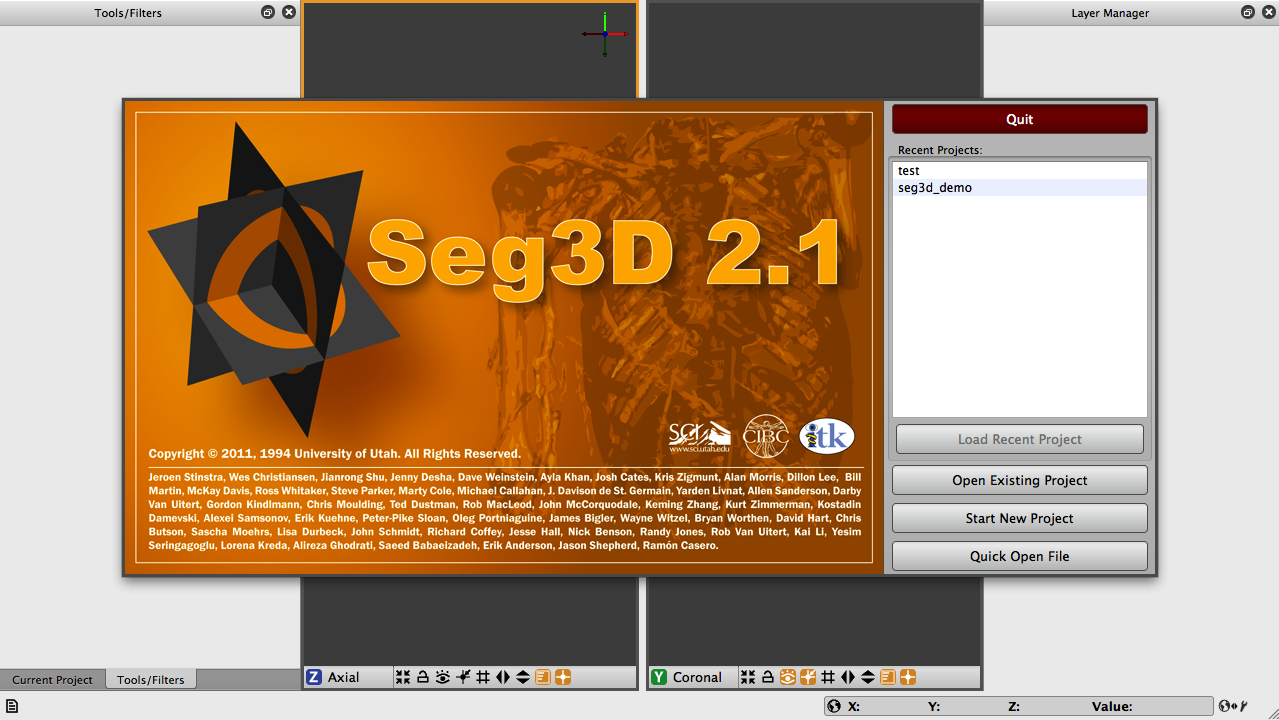
\includegraphics{Seg3DTutorial_figures/welcome_screen.png}}
%\caption{Seg3D welcome screen}\label{fig:welcome}
%\end{figure}

\chapter{Seg3D Viewer}

\begin{introduction}

\end{introduction}

\section{2D Slice Viewer}

\section{3D Volume Viewer}

\section{Viewing Options}

\chapter{Seg3D Windows}

\begin{introduction}
In addition to the viewer windows discussed in the above chapter, there are several other
 windows involved in streamlining the user interface of the Seg3D software.  
 Each of these windows can be accessed through the 'Window' dropdown menu.
 By default these windows appear in certain positions defined below, but each can be undocked
 from the Seg3D interface and either left as stand alone windows or repositioned elsewhere on
 the Seg3D application.
  
\end{introduction}

\section{Project Window}

\begin{figure}
\scalebox{0.3}{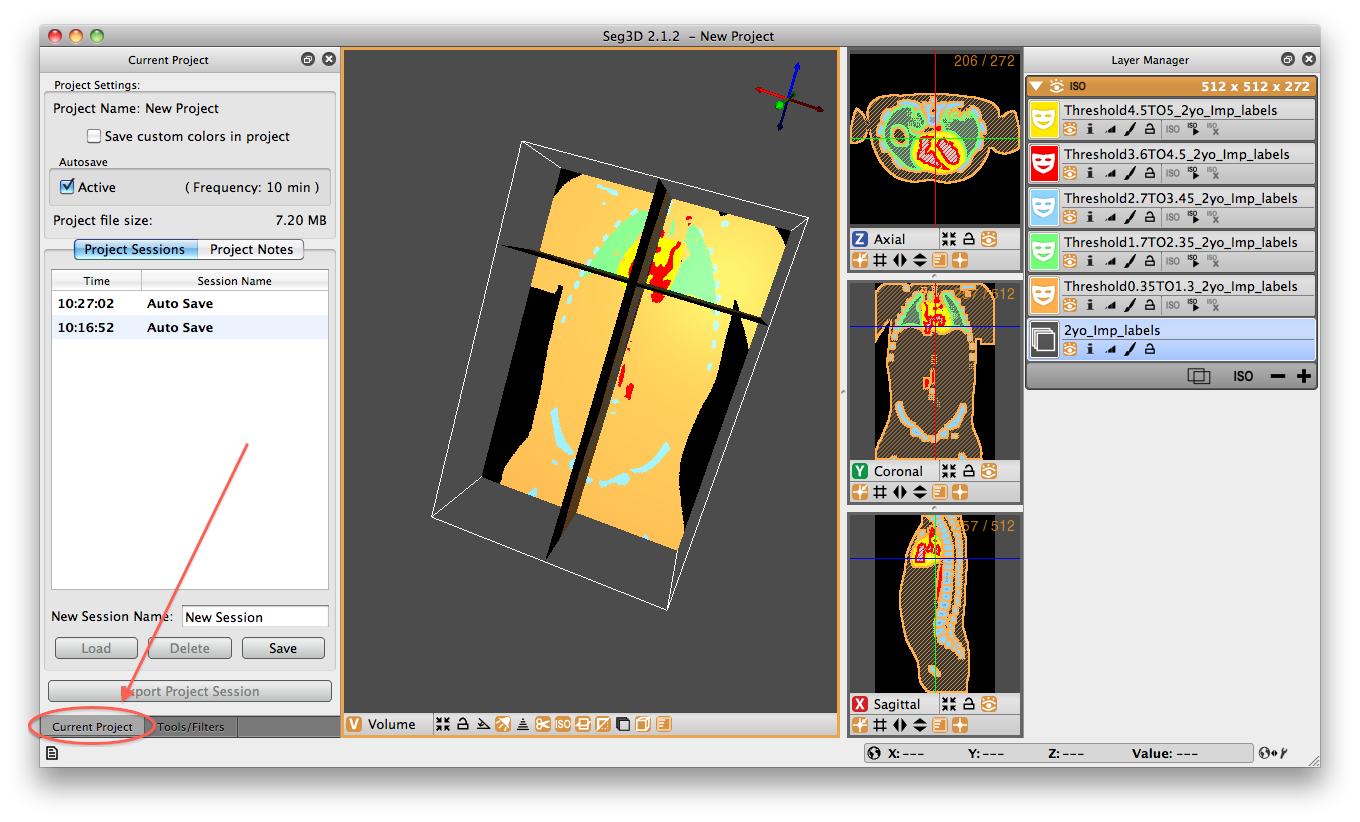
\includegraphics{Seg3DTutorial_figures/ProjectWindow.png}}
\caption{Project Window}\label{fig:ProjectWindow}
\end{figure}
The project window is one of three windows that is opened by default when Seg3D launches.  
It is located on the left side of the panel and is secondary to the default 'Tools Window' which is also 
located on the left but appears over top of the project window.  
In order to access the window, simply click the tab at the bottom of the left side named 'Current Project' (See Figure \ref{fig:ProjectWindow}) or go to the 'Window' drop down menu, de-select 
'Project Window' and reselect it.

Now you come to the 'Current Project' window.  
The window is divided into two panes.  
At the top of the window is the Project Settings pane.  
The name of the current project is listed.  
Below this is the option to 'Save custom colors in project.'  
This option allows the user to keep the defined colors assigned to specific label masks within the project.  
Below this is an 'Autosave' option. Seg3D autosaves sessions every 10 minutes by default.  
The default time between autosaves can be changed in the general Seg3D preferences.

The second pane holds the 'Project Sessions' and 'Project Notes' panels.  
The project session contains information on the saving of various sessions throughout the worktime in Seg3D - including autosaves.  
These session saves can be selected and loaded at any time.  
Loading a session save does not delete saves that came later.  
To delete, the user must explicitly select the session and push the delete button at the bottom of the pane.  
Additional sessions may also be saved with user specified names.  
The second panel of this pane (the 'Project Notes' panel) allows the user to write notes to along the way.

At any time the user can export the session to a new location - with or without a different name than the original session by clicking the 'Export the Project Session button on the bottom of the  'Current Project' window.

\section{Tools Window}
\begin{figure}[b]
\scalebox{0.3}{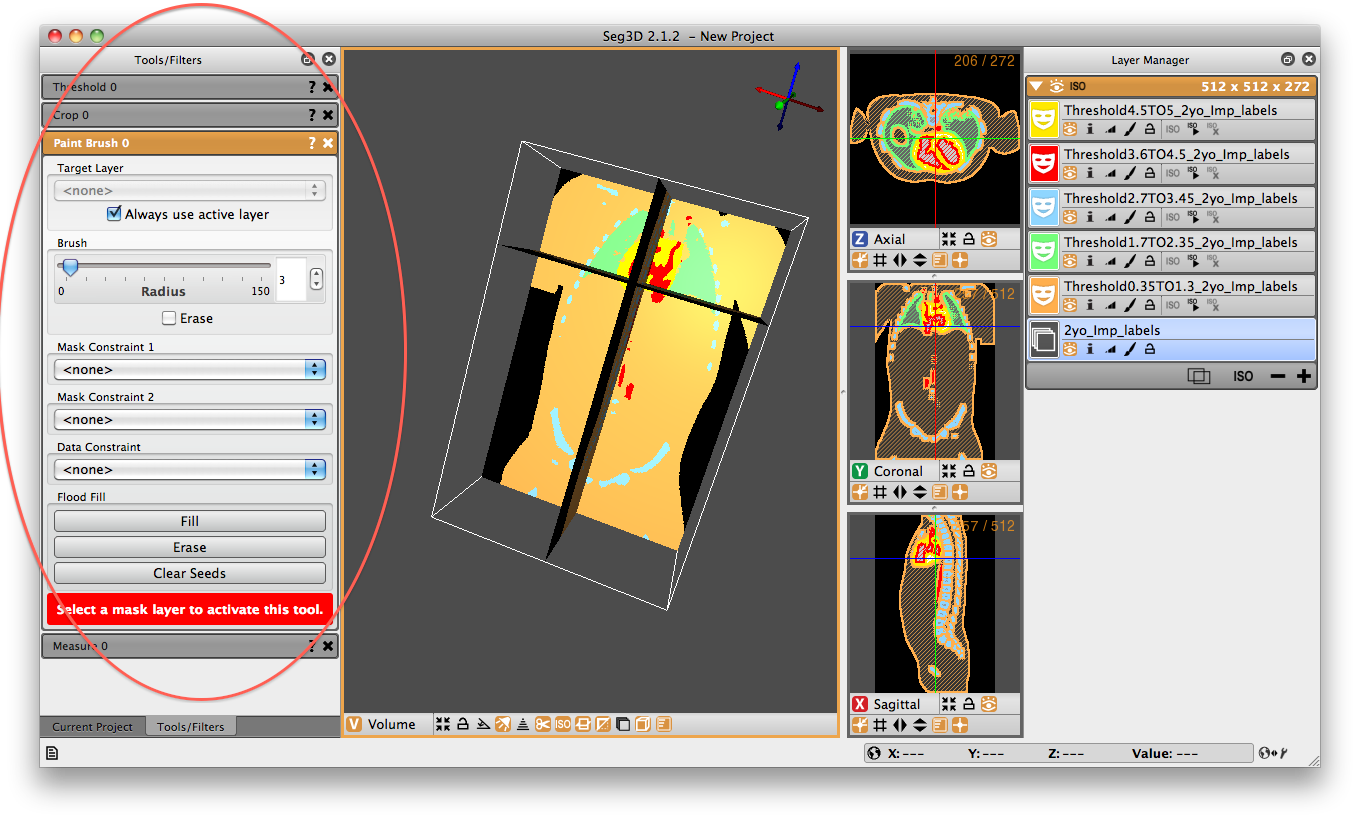
\includegraphics{Seg3DTutorial_figures/ToolWindow.png}}
\caption{Tools Window}\label{fig:ToolWindow}
\end{figure}
The tools window is another of the three windows that is opened upon Seg3D launch.  
This window is also on the left of the Seg3D panel and is, unlike the project window, is displayed when Seg3D is opened.  
Users can toggle between project and tool windows by selecting the specific tabs at the bottom of the left most window pane.

The tool window houses the current tools that the user has selected from the 'Tools' dropdown menu.  
The active tool will be highlighted in orange and will be displayed.  
Inactive tools, that have been opened during the session, will be grayed out and minimized.  
To access one of the other tools, click one of the grayed out items or select it from the 'Tools' dropdown menu.  
In Figure \ref{fig:ToolWindow} the 'Paint Brush' tool is active, while the 'Threshold,' 'Crop,' and 'Measure' tools are inactive.



\section{Layer Manager Window}
The layer manager window is the last of the three windows that open by default upon launching Seg3D.  
This window is positioned to the right side of the Seg3D window pane and contains all of the mask and volume files involved with the session.  
If a file is not selected when Seg3D launches, this window will be blank, otherwise it will contain the volume and mask surface files associated with the opened file.

\begin{figure}[b]
\scalebox{0.3}{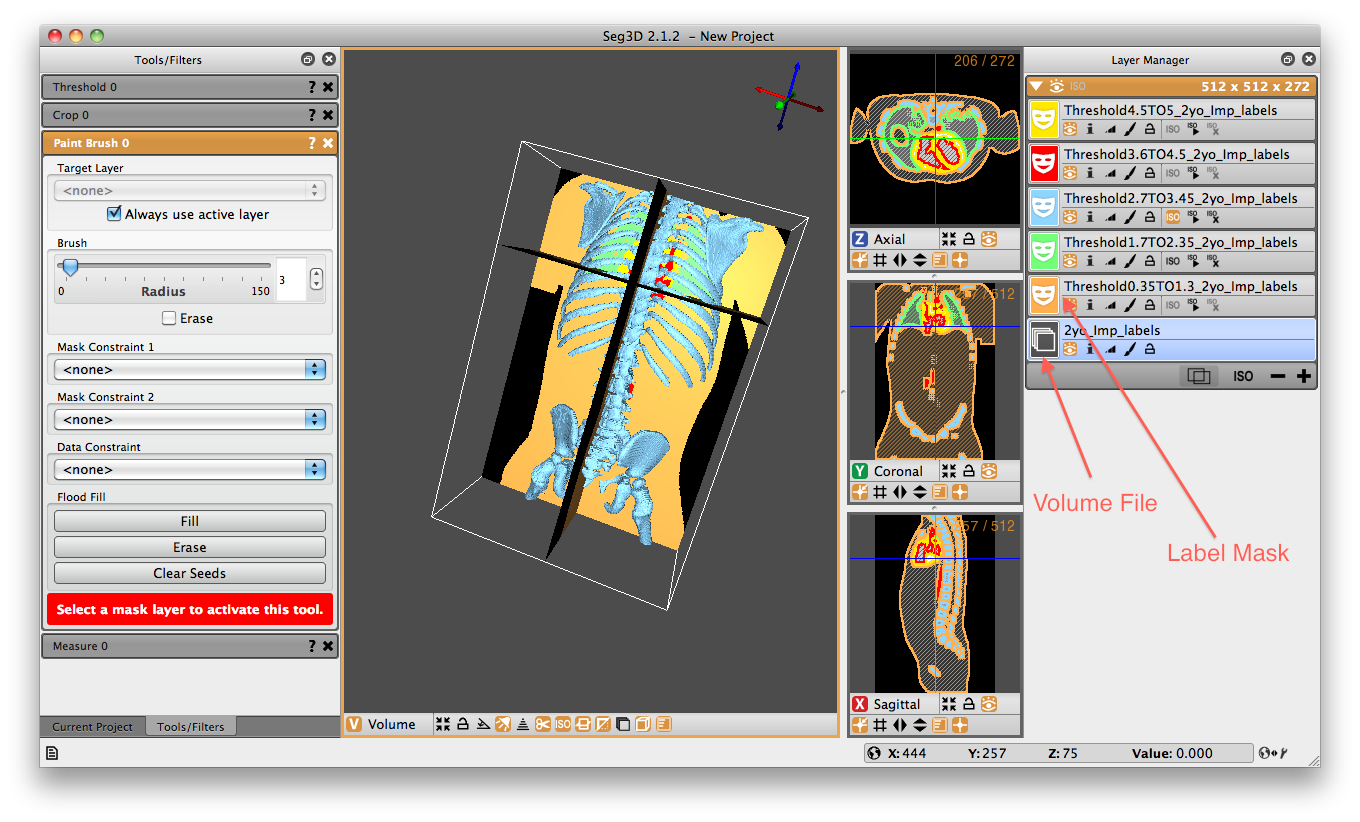
\includegraphics{Seg3DTutorial_figures/LayerWindow.png}}
\caption{Layer Manager Window}\label{fig:LayerWindow}
\end{figure}

A volume file is represented by a gray image with multiple stacked planes.  
A label mask is represented by a colored icon with a white mask in the middle.  
The colors correspond to the label masks seen in the viewer windows.
Names of label masks are, by default, a conglomeration of the tools applied to the original volume.
For example, in the image Figure \ref{fig:LayerWindow} five label masks have been created from the volume file '\verb|2yo_Imp_labels|.' 
The uppermost mask (in yellow) has the name '\verb|Threshold4.5TO5_2yo_Imp_labels|.' 
This name was generated because the threshold tool, with values between 4.5 and 5, was applied to the original volume file. 
If another tool were to be applied on the yellow mask, the new mask would state the name of the tool, followed by the complete name of the yellow label mask.  
Names of masks can be manually changed by clicking the current name and typing in the desired text.

Each volume or mask label has  standard, associated icons below their names.
A brief description of each icon follows:

%% insert figure  of the eye
\begin{figure}[h!]
  
\includegraphics[width=0.05\textwidth]{Seg3DTutorial_figures/VisibleOff.png}% picture filename
  \caption{Visible Icon: The eye icon displays the current mask.  When the eye is highlighted the mask is visible in the view plane, when it is not, the mask is 'turned off.'}
\end{figure}


%% insert figure of the 'i'
\begin{figure}[h!]
  
\includegraphics[width=0.05\textwidth]{Seg3DTutorial_figures/InfoOff.png}% picture filename
  \caption{Info Icon: The 'i' icon displays information about the layer.}
\end{figure}

%% insert figure of the bar chart
\begin{figure}[h!]
  
\includegraphics[width=0.05\textwidth]{Seg3DTutorial_figures/OpacityOff.png}% picture filename
  \caption{Opacity Icon: The histogram-looking icon allows the user to change opacity levels of the layer.}
\end{figure}

%% insert figure of the paintbrush
\begin{figure}[h!]
  
\includegraphics[width=0.05\textwidth]{Seg3DTutorial_figures/AppearanceOff.png}% picture filename
  \caption{Appearance Icon: The paintbrush-like icon allows the user to change the layer's appearance.}
\end{figure}

%% insert figure of the lock
\begin{figure}[h!]
  
\includegraphics[width=0.05\textwidth]{Seg3DTutorial_figures/LockOff.png}% picture filename
  \caption{Lock Icon: The lock icon allows users to lock the layer to further editting.}
\end{figure}

%% insert figure of 'ISO'
\begin{figure}[h!]
  
\includegraphics[width=0.05\textwidth]{Seg3DTutorial_figures/IsosurfaceMenuOff.png}% picture filename
  \caption{IsosurfaceMenu Icon: This icon displays active isosurfaces (if the mask has one).}
\end{figure}

%% insert figure of ISO playbutton
\begin{figure}[h!]
  
\includegraphics[width=0.05\textwidth]{Seg3DTutorial_figures/IsosurfaceComputeOff.png}% picture filename
  \caption{IsosurfaceCompute Icon: This icon generates the isosurface for the mask.  It must be clicked before the IsosurfaceMenu or IsosurfaceDelete icons become active.}
\end{figure}

%% insert figure of ISO x
\begin{figure}[h!]
  
\includegraphics[width=0.05\textwidth]{Seg3DTutorial_figures/IsosurfaceDeleteOff.png}% picture filename
  \caption{IsosurfaceDelete Icon: This icon deletes active isosurfaces (if the mask has one).}
\end{figure}

These icons represent tools that are available for each individual layer.  
Additionally, features of these masks can be toggled universally by clicking similar icons on the top of the pane, in the orange bar.  
Hovering the cursor over the icon will display the the use of each additional icon.

At the bottom of the pane, options are provided to allow the user to: 
\begin{itemize}
\item Duplicate a layer
\item Change isosurfacing settings
\item Delete a layer
\item Add a layer
\end{itemize}


\section{Volume View Window}
The Volume View Window is not opened by default when Seg3D is opened.  
To open the window, click the 'Window' option in the task bar and select the Volume View option.  
The window may also be toggled by using the key command: Shift+cntrl/cmd+V. 
Once activated, the window will appear on the right and side of the Seg3D panel covering the layer mask window.
To toggle back to the layer mask window, click the Layer Manager tab at the bottom of the page.
The Volume View Window has three separate options for volume displaying.



\subsection{Fog Panel}



The Fog Panel allows the user to control the fog density.  
In order to observe the effects of fog, the user must activate the Show fog icon on the bottom of the 3D viewer window.
Once active, a fog will be observed on the image.  
The depth of the fog is determined by the distance that the 3-dimensional component is away from the viewer.   
In Figure \ref{fig:FogPanel} the pelvis is tilted away from the viewer.
It is therefore farther from the viewer and has more fog effect applied to it.

Fog density can be tuned by using the slider in the the Volume View Window.  
By default the density value is 1.00.
If the fog density increases, the fogging effect increases.
\begin{figure}[t]
\scalebox{0.3}{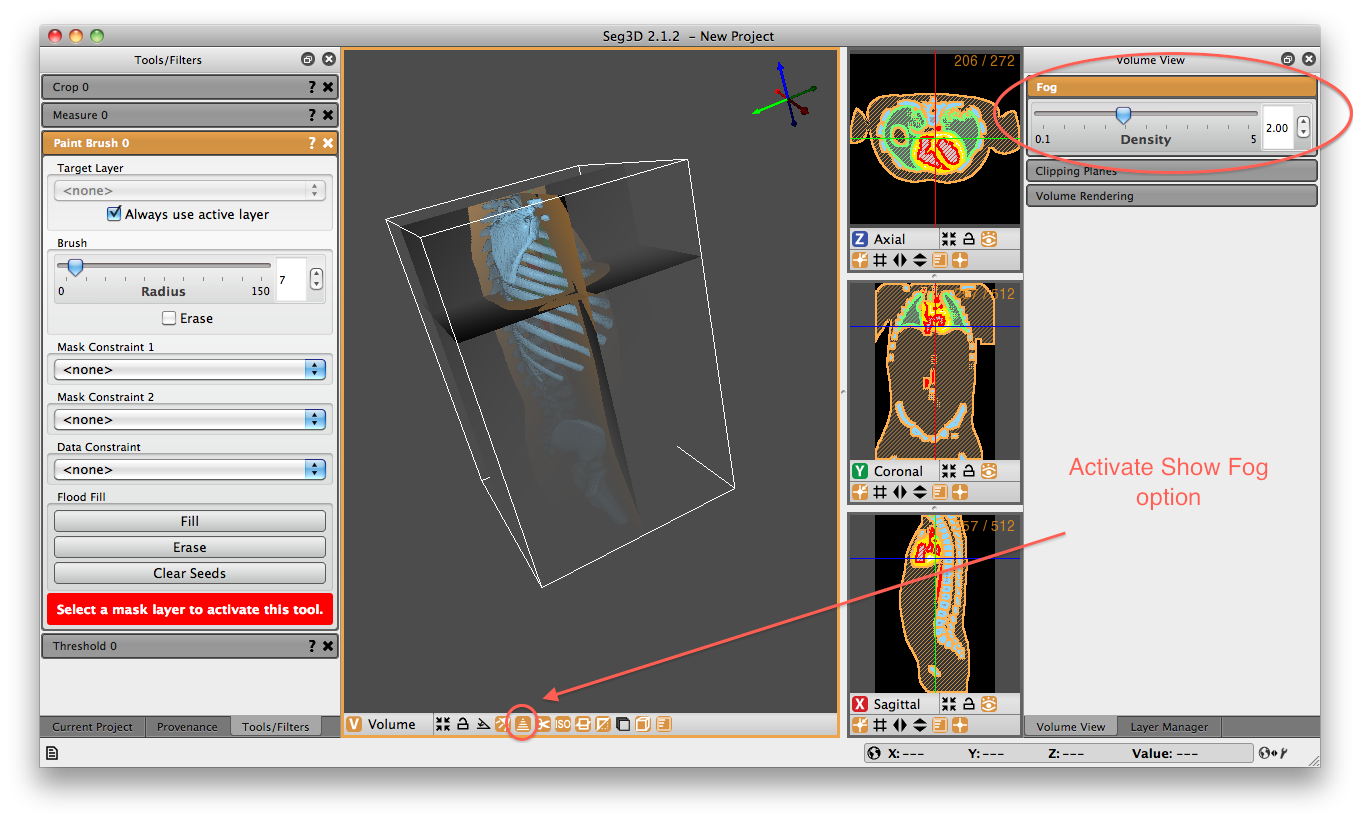
\includegraphics{Seg3DTutorial_figures/FogPanel.png}}
\caption{Volume View Window - Fog Panel Displayed. The user must activate the Show fog option at the bottom of the viewer window.}\label{fig:FogPanel}
\end{figure}

\subsection{Clipping Planes Panel}
The Clipping Planes Panel allows users to define multiple clipping planes with which to clip the volume.  
+ and - signs at the top of the panel represent individual clipping planes.  
The + sign is an enabled clipping plan, while the - sign is disabled.
The clipping panel option in the viewer window is activated by default.

\begin{figure}[b!]
\scalebox{0.3}{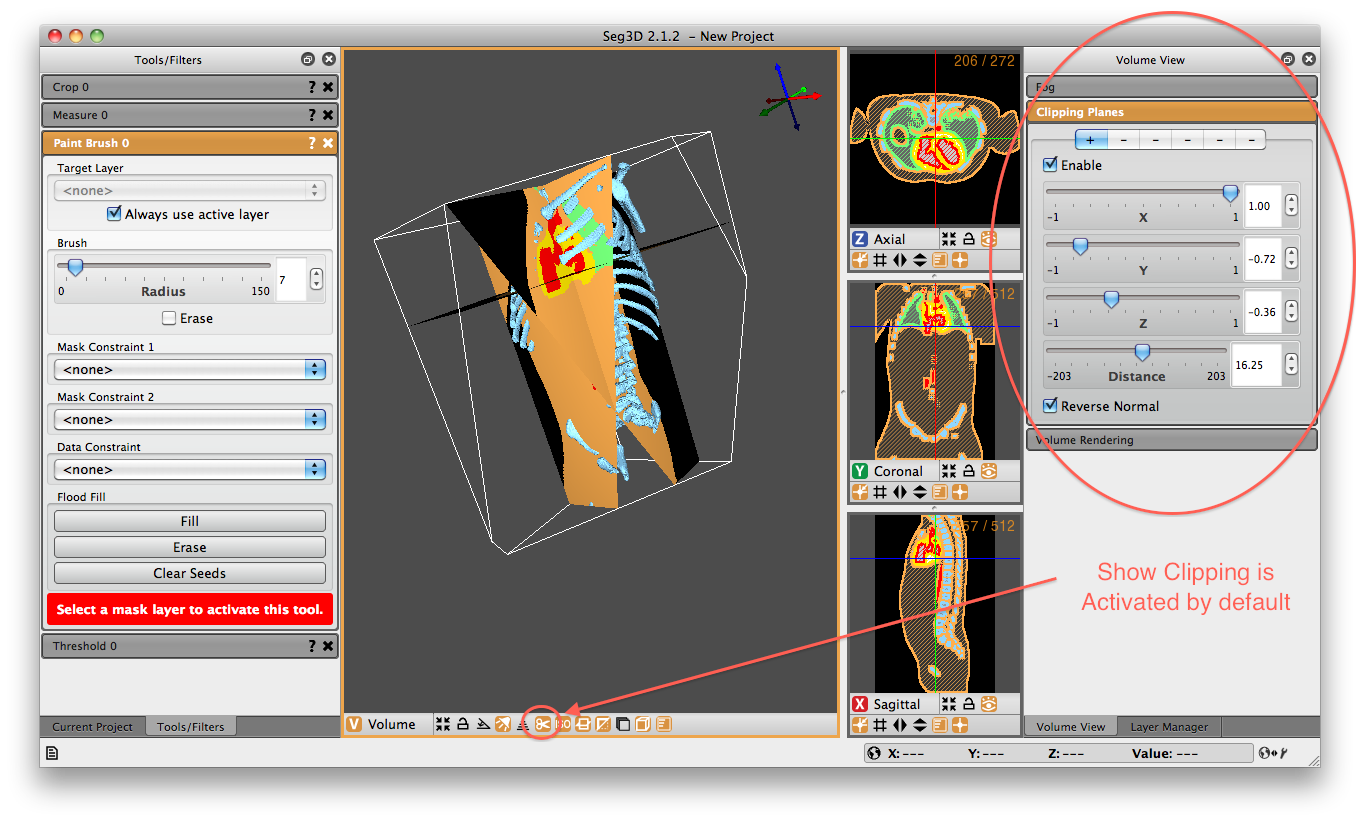
\includegraphics{Seg3DTutorial_figures/ClippingPanel.png}}
\caption{Volume View Window - Clipping Panel Displayed. Show clipping option at the bottom of the viewer window is activated by default.}\label{fig:ClippingPanel}
\end{figure}

Once an clipping plane has been selected, it must be enabled.  Click the 'Enable' checkbox.  
After the plane is enabled, the user is able to define the influence of each cardinal direction on the plane.  
The number 1 in a box indicates that the clipping plane will slice a 45-degree angle within the positive side of that cardinal direction on the 3d viewing window. 
A -1 will clip a -45-degree angle from the negative side.

In order to activate a clip from any cardinal direction, the user must click the slider associated with the desired plane.
If the slider is not clicked, no clipping will take place...even with the clipping plane enabled.
If, say, the z slider is not clicked, no clipping will occur in that plane.
Combining these directional clips allows the user to define a plane that is tipped and tilted in any 3-dimensional direction.
A fourth slider option, the Distance slider, allows the user to define how the position of the clipping plane with respect to the volume.  
If the distance slider is set all the way to the left, no image will be displayed (it will be completely clipped).
If it is set to the right, the entire image will be displayed (no clipping is applied).  
Anything in between will show some clipping of the image.

The final option in the Clipping Planes panel is the option to 'Reverse Normal.'
This option allows the user to reflect the clipping plane.
That is, if the image is clipped within the positive XY plane, the 'Reverse Normal' option will display the clip within the negative XY plane
Figure \ref{fig:ClippingPanel} shows the result of a clipping plane applied in all three cardinal directions.

\subsection{Volume Rendering Panel}

\begin{figure}[b!]
\scalebox{0.3}{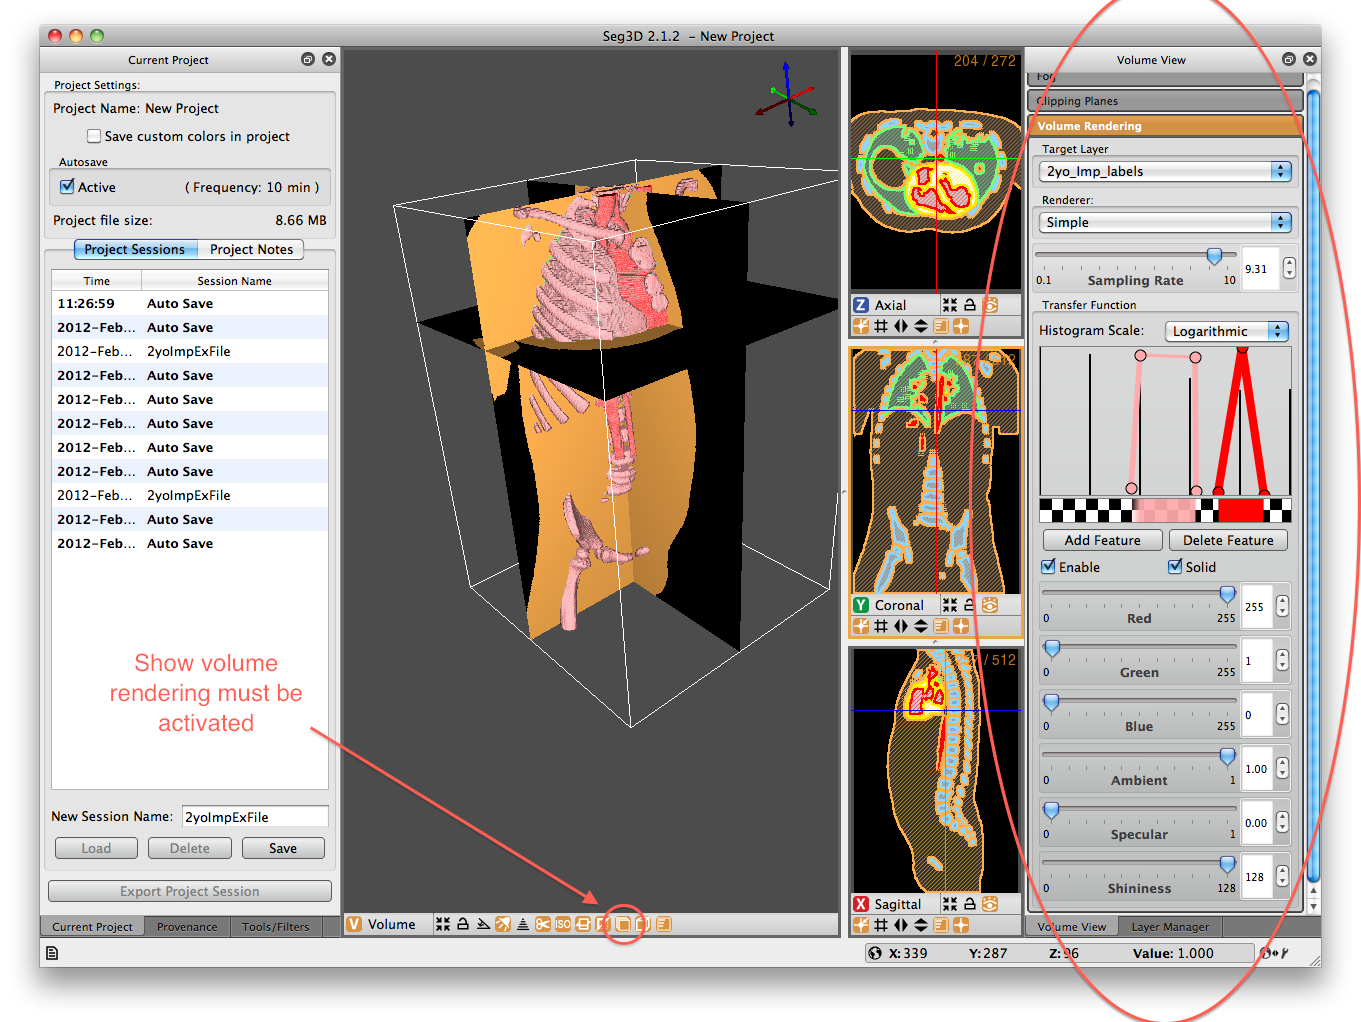
\includegraphics{Seg3DTutorial_figures/VolRendPanel.png}}
\caption{Volume View Window - Volume Rendering Panel Displayed. Show volume rendering icon at the bottom of the viewer window must be activated.}\label{fig:VolRendPanel}
\end{figure}

The volume rendering panel allows users to generate a volume directly from the volume file, based on the application of transfer functions.
These volume representations are created by extracting values from the transfer functions available and displaying them on a slice-by-slice basis.
If the user zooms the image in closely, each individual slice can be seen (Figure \ref{fig:VolRendOpt}).
The user must define the volume over which they would like to perform the volume rendering.
The user must also make sure that the 'show volume rendering' option is selected at the bottom of the 3D viewer window.

\subsection{Rendering options}

With these two options selected, the user now has three rendering options.
These options are Simple, Faux Shading, and Ambient Occlusion.

\begin{figure}[h!]
\scalebox{0.3}{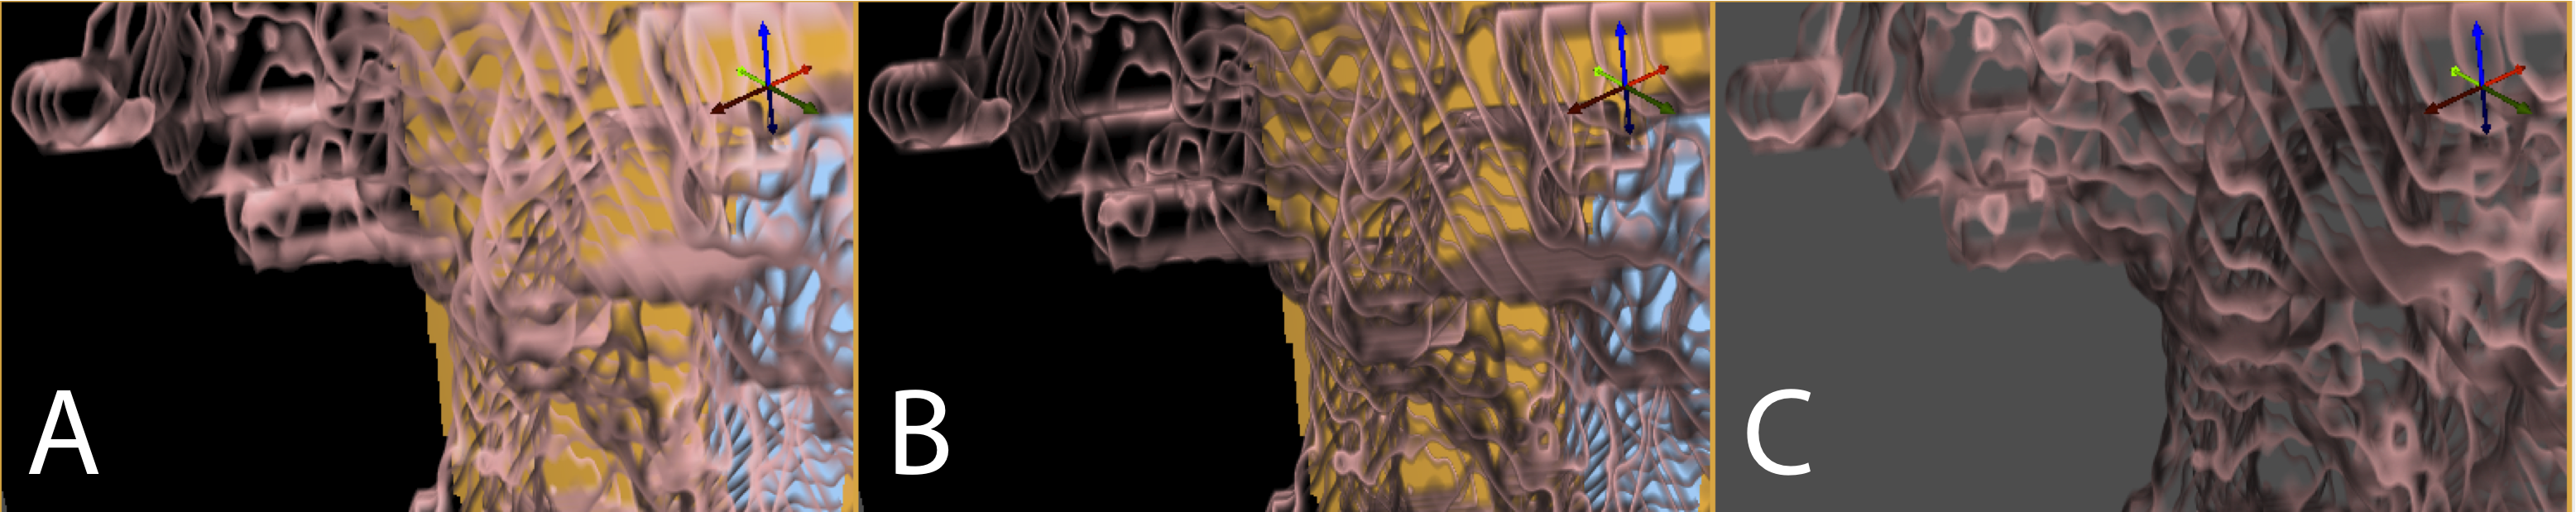
\includegraphics{Seg3DTutorial_figures/VolRendOpt.png}}
\caption{Volume Rednering Options - A) Simple B) Faux Shading C) Ambient Occlusion}\label{fig:VolRendOpt}
\end{figure}

\subsubsection{Simple}
The simple rendering strategy gives the user the option to select the Sapling Rate.
The higher the rate, the more accurate the representation of the selected region.
An option in the 'Transfer Function' section of the pane that allows the user to choose 'Solid' transfer function representation changes the appearance by coloring each selected slice to a solid color.
More on this feature will be addressed below.
Note that the images in Figure \ref{fig:VolRendOpt} do not have the solid option selected.

\subsubsection{Faux Shading}
Faux Shading is the same as the simple rendering option with the exception that a simple shading is added to the visible volume.
Where the simple rendering fades regions of the slice to clear (where the 'Solid' transfer function option is NOT selected), the Faux Shading options fade slices to a grayer hue, dependent on where it sits from other 3-dimensionally viewed volumes.
If the 'Solid' feature is selected, the Simple and Faux Shading rendering are the same.

\subsubsection{Ambient Occlusion}
Ambient Occlusion has several additional options.
In addition to the sampling rate, an occlusion angle (range: 0 to 80 degrees) and a sample resolution (range: 1 to 10) are now available.

%Not sure what is these additional options mean.
%The Sample Rate determines the general resolution of the volume.
%The Sample Resolution and the Occlusion angle determine


\subsection{Transfer Function}
Within the transfer function pane, a histogram exists that defines the volumetric image.
The transfer function can be displayed on a Linear or Logarithmic scale.
In the transfer function window, the user can choose to add or delete a feature.
A feature can be dragged into positions defining regions of the histogram that the user wants to render.
The default Feature is a line.  
By clicking and dragging the line, the feature can be moved.
By clicking a point on the line, the individual point can be moved.
Additional points can be added to a feature by clicking anywhere in the histogram panel  that is not already defined by a line, that is, in the gray or black regions.

Each of the features observed can also be enabled/disabled and viewed as solid or graded.
The solid feature (as addressed above) allows the feature to be represented as a graded slice or as a solid one.
Solid slices simply apply the same color saturation to each section of the volume slice.
De-selecting the solid option applies a gradient to the slices, with the outer edge being the brightest color.

Each point and feature can be repositioned, reshaped, and recolored in order to distinguish between defined regions.
To change the color of a feature, select the desired feature and adjust the slider regions below the histogram in the Red/Green/Blue features.
Colors can be used to easily distinguish different features in the volume.
Additionally, each features Ambient and Specular lighting can be adjusted as well as volume shininess is adjustable



\section{Provenance Window}
The Provenance Window is not opened by default when Seg3D is opened. 
To open the window, click the 'Window' option in the task bar and select the Provenance option.  
The window may also be toggled by using the key command: Shift+cntrl/cmd+H.
When the window opens, it will appear on the left side of the Seg3D user interface over top of the 'Current Project' panel and the 'Tools' panel.

The Provenance Window shows the history of the active layer.  
In order to see which actions lead to the current layer, highlight the layer in the 'Layer Window' on the left of the Seg3D display.
Initially, nothing will appear in the Provenance window.
Click the Refresh button at the bottom of the panel and the complete history of that mask will appear.

\begin{figure}[b!]
\scalebox{0.3}{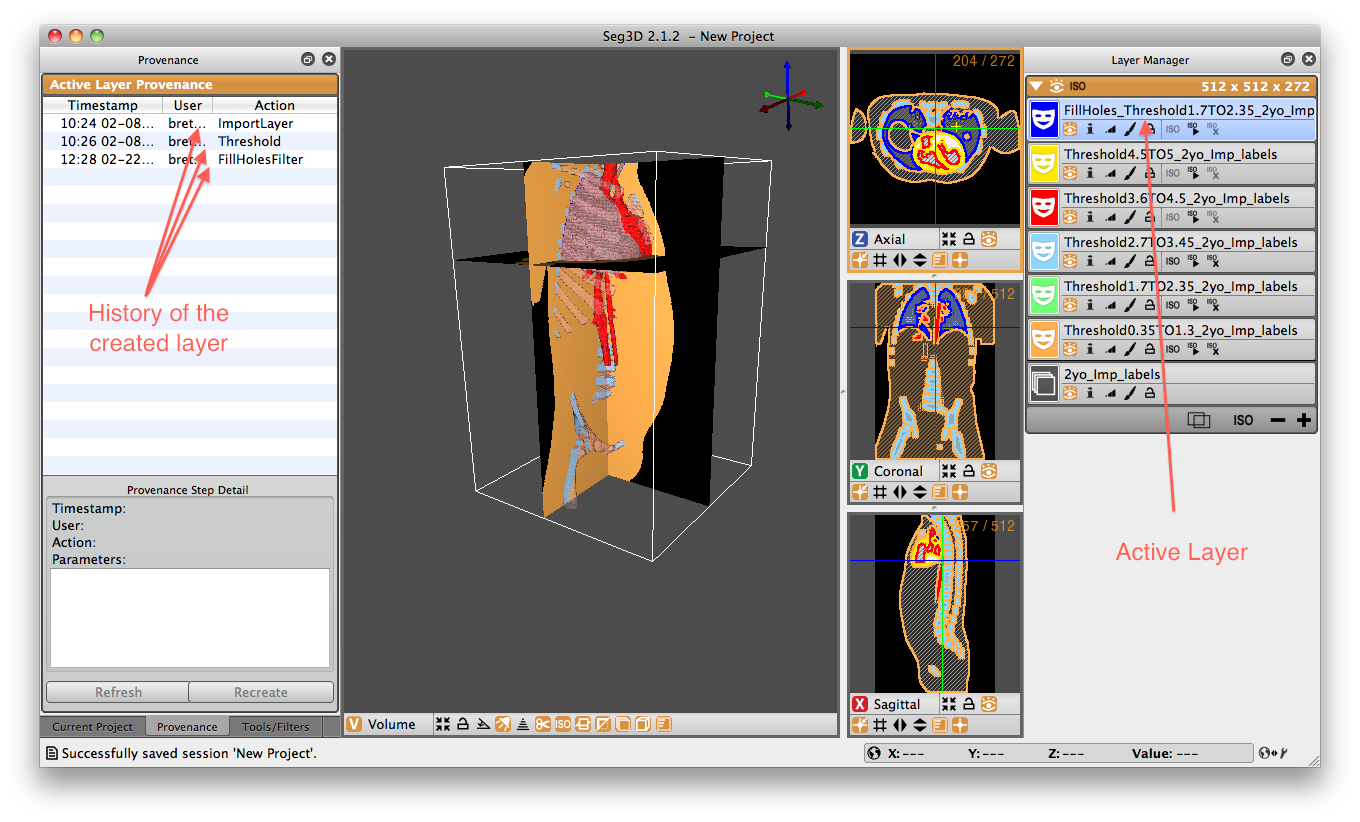
\includegraphics{Seg3DTutorial_figures/ProvenanceWindow.png}}
\caption{Volume View Window - Clipping Panel Displayed. Show clipping option at the bottom of the viewer window is activated by default.}\label{fig:ProvenanceWindow}
\end{figure}

For example, Figure \ref{fig:ProvenanceWindow} shows an example of a 'FillHoles' Layer.
This layer was was generated by applying a FillHoles tool to the thresholded mask of the lungs.
As can be seen in the Provenance panel, the first step in creating this mask was to Import the volume layer.  
Next, a threshold was taken.  Last, the FillHolesFilter was applied to the Threshold mask.
By selecting one of the steps in the Provenance window, the parameters defining that portion of the mask history will be shown.
For example, by selecting the Threshold option, the thresholding range will be displayed.

\section{Controller Window}
The Controller Window is not opened by default when Seg3D is opened.  To open the window, click the 'Window' option in the task bar and select the Controller option.  The window may also be toggled by using the key command: Shift+cntrl/cmd+C.
Notice the Controller Window option in the window drop-down menu is located below a seperator.  
This indicates that the window will open a new pop-up window outside of the general Seg3D user interface.

The Controller window supplies the user with all of the data, variables, history, and logs of the current Seg3D session.
There are four tabs that can be selected in this window:

\subsection{Actions Tab}
The action tab displays all of the actions that have been taken during the Seg3D session.
Console entries can also be made with this feature.
A series of actions area provided in a dropdown menu at the bottom of the window.
Once selected, the action will be placed into a command line to the right of the dropdown menu.
The user can then define the parameters for the action, or simply press enter to see what parameters are required to make the action valid.
If additional parameters are needed to run the action, they will be displayed in the box below the command line.

\subsection{State Variables Tab}
The state variables tab  shows a list of all the state settings for the session.
Settings cannot be edited in this window.

\subsection{Event Log Tab}
The event log shows actions that have been taken on the session since the latest load of the session.
If Seg3D is closed, and then reopened, the event log will only record the history for the newly opened session.
This differs from the action tab in this way, which collects actions for the entire history of the session.
The event log also differs from the action log in that it records all events involved with running Seg3D, not just the actions.
This is also a non-editable tab.

\subsection{Undo/Redo Buffer Tab}
The Undo/Redo Buffer stores past actions for the current open project.
Closing the session will erase the buffers.
In these buffers a user can find the actions, in order, than can be either undone or redone by using Seg3D's Undo and Redo options.


\section{Python Console}
The Python Window is not opened by default when Seg3D is opened.  To open the window, click the 'Window' option in the task bar and select the Python option.  The window may also be toggled by using the key command: Shift+cntrl/cmd+Y.
Notice the Python Window option in the window drop-down menu is located below a seperator.  
This indicates that the window will open a new pop-up window outside of the general Seg3D user interface.

The Python Window opens a python scripting console that can be used by advanced users to editing the Seg3D data via python coding.  
A treatment of python coding will not be attempted in this document.
For more information on python coding, consult other resources.

\chapter{Basic Program Functions}

\begin{introduction}

\end{introduction}

\section{File}

\subsection{New Project}

\subsection{Open Project}

\subsection{etc.}

\section{Edit}

\section{Help}

\section{Preferences}

\chapter{Tools \& Filters}

\begin{introduction}

\end{introduction}

\section{Tools}

\subsection{Copy/Paste}

\subsection{Crop}

\subsection{etc.}

\section{Mask Filters}

\subsection{etc.}

\section{Data Filters}

\subsection{etc.}

\section{Advanced Filters}

\subsection{etc.}

\end{document}

